% !TEX spellcheck = en_US



% ~~~~~~~~~~~~~~~~~~~~~~~~~~~~~~~~~~~~~~~ V
% (NC) 2026 Haluk Bingol
% github.com/halukbingol/LaTeX-Templates
%
% Licensees may copy, distribute, display, and perform the work and make derivative works 
% and remixes based on it only for non-commercial purposes. 
% ~~~~~~~~~~~~~~~~~~~~~~~~~~~~~~~~~~~~~~~ A




% =====================================================================
%  Stacks -- Junior Level: Performance, Memory and the Call Stack
%  ---------------------------------------------------------------------
%  Built on hblib/Template/hblibTemplate.tex with the libraries in ../../hblib/.
%  Programs and their real outputs are in codeoutput/:
%     codeoutput/<Name>.java  a program (classes without main() are only compiled)
%     codeoutput/<Name>.sh    a terminal session, run in a copy of codeoutput/<Name>/
%     codeoutput/<Name>.txt   what it printed, made by:  bash run_examples.sh
% =====================================================================

\documentclass[aspectratio=169,10pt,compress]{beamer}

% ~~~~~~~~~~~~~~~~~~~~~~~~~~~~~~~~~~~~~~~~~~~~~~~~~~~~~~~~~~~~~~~~~ V hblib
	\usepackage{../../hblib/hblibPresentation} % lib presentation: theme, i/N, \hSection, algorithm2e, ...
	\usepackage{../../hblib/hblibCodeoutput} % lib code + output: \lstcode, \lstterminal, ...
	\usepackage{../../hblib/hblibDatastructures} % lib data structures: \hString, \hStack, \hQueue
% ~~~~~~~~~~~~~~~~~~~~~~~~~~~~~~~~~~~~~~~~~~~~~~~~~~~~~~~~~~~~~~~~~ A hblib


% xcolor, array (and the L{width} column), listings, tikz and algorithm2e come from the hblib libraries
\usepackage[T1]{fontenc}
\usepackage{lmodern}
\usepackage{booktabs}

\newcommand{\win}{\textbf{Windows}}
\newcommand{\mac}{\textbf{macOS}}

% algorithm2e set-up (the package is loaded by hblibPresentation)
\SetAlCapFnt{\small}
\SetAlCapNameFnt{\small}
\SetKwProg{Fn}{function}{}{end}
\SetKw{KwError}{error}

% ---------------------------------------------------------------------
\title{Stacks}
\subtitle{Junior Level: Performance, Memory and the Call Stack}
\author[Bingol]{Haluk O. Bingol}

\institute[FCIS]{
    Faculty of Computer and Information Sciences\\
    Yeditepe University
}
\date{
	{\tiny \hbTimeStamp}
}

\begin{document}




% ~~~~~~~~~~~~~~~~~~~~~~~~~~~~~~~~~~~~~~ V frm
\begin{frame}[t,fragile]
  \titlepage
\end{frame}
% ~~~~~~~~~~~~~~~~~~~~~~~~~~~~~~~~~~~~~~ A frm




% ~~~~~~~~~~~~~~~~~~~~~~~~~~~~~~~~~~~~~~ V frm
\begin{frame}[t,fragile] \frametitle{Outline}
  \begin{columns}[T]
    \begin{column}{0.48\textwidth}
      \tableofcontents[sections={1-3}, hideallsubsections]
    \end{column}
    \begin{column}{0.48\textwidth}
      \tableofcontents[sections={4-6}, hideallsubsections]
    \end{column}
  \end{columns}
\end{frame}
% ~~~~~~~~~~~~~~~~~~~~~~~~~~~~~~~~~~~~~~ A frm

% ~~~~~~~~~~~~~~~~~~~~~~~~~~~~~~~~~~~~~~ V
\hSection[Implementations]{Array or Linked List?}
% ~~~~~~~~~~~~~~~~~~~~~~~~~~~~~~~~~~~~~~ A




% ~~~~~~~~~~~~~~~~~~~~~~~~~~~~~~~~~~~~~~ V frm
\begin{frame}[t,fragile] \frametitle{A linked stack}
  \begin{columns}[T]
    \begin{column}{0.49\textwidth}
      \lstcode[basicstyle=\ttfamily\tiny, lastline=17]{codeoutput/LinkedStack.java}{Java}
    \end{column}
    \begin{column}{0.49\textwidth}
      \lstcode[basicstyle=\ttfamily\tiny, firstline=18, firstnumber=18]{codeoutput/LinkedStack.java}{Java}
    \end{column}
  \end{columns}
\end{frame}
% ~~~~~~~~~~~~~~~~~~~~~~~~~~~~~~~~~~~~~~ A frm




% ~~~~~~~~~~~~~~~~~~~~~~~~~~~~~~~~~~~~~~ V frm
\begin{frame}[t,fragile] \frametitle{How the linked stack works}
  \begin{center}
  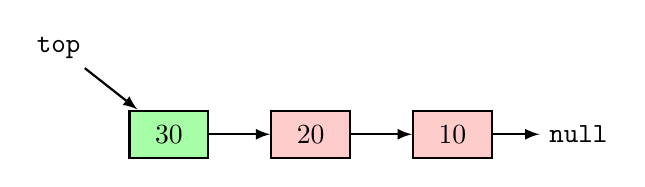
\begin{tikzpicture}[nd/.style={draw, thick, minimum width=1cm, minimum height=0.6cm}]
    \node[font=\ttfamily] (t) at (-0.6,1.1) {top};
    \node[nd, fill=green!35] (c) at (0.8,0) {30};
    \node[nd, fill=red!20]   (b) at (2.6,0) {20};
    \node[nd, fill=red!20]   (a) at (4.4,0) {10};
    \node[font=\ttfamily] (n) at (6.0,0) {null};
    \draw[-latex, thick] (t) -- (c);
    \draw[-latex, thick] (c) -- (b);
    \draw[-latex, thick] (b) -- (a);
    \draw[-latex, thick] (a) -- (n);
  \end{tikzpicture}
  \end{center}
  \begin{itemize}
    \item push: a new node in \textbf{front}, pointing to the old top; pop: \texttt{top = top.next}.
    \item Never full, never copies: $O(1)$ \textbf{worst case} for every operation, not just amortized.
    \item But one extra object (the \texttt{Node}) per element: more memory, more work for the garbage collector.
    \item \texttt{static} nested class: a \texttt{Node} does not need a reference to its stack.
  \end{itemize}
\end{frame}
% ~~~~~~~~~~~~~~~~~~~~~~~~~~~~~~~~~~~~~~ A frm




% ~~~~~~~~~~~~~~~~~~~~~~~~~~~~~~~~~~~~~~ V frm
\begin{frame}[t,fragile] \frametitle{Two primitive-friendly stacks}
  \begin{columns}[T]
    \begin{column}{0.52\textwidth}
      \lstcode[basicstyle=\ttfamily\tiny]{codeoutput/IntArrayStack.java}{Java}
    \end{column}
    \begin{column}{0.44\textwidth}
      \begin{itemize}\small
        \item \texttt{ArrayStack<Integer>} stores \textbf{references} to \texttt{Integer} objects (boxing).
        \item \texttt{IntArrayStack} stores the \texttt{int} values themselves, next to each other.
        \item The JDK has no primitive collections; libraries such as Eclipse Collections or fastutil do.
        \item Project Valhalla (value classes) aims to remove much of this cost in future Java versions.
      \end{itemize}
    \end{column}
  \end{columns}
\end{frame}
% ~~~~~~~~~~~~~~~~~~~~~~~~~~~~~~~~~~~~~~ A frm

% ~~~~~~~~~~~~~~~~~~~~~~~~~~~~~~~~~~~~~~ V
\hSection[Performance]{Measuring Performance}
% ~~~~~~~~~~~~~~~~~~~~~~~~~~~~~~~~~~~~~~ A

% ~~~~~~~~~~~~~~~~~~~~~~~~~~~~~~~~~~~~~~ V
\subsection[Time]{Time}
% ~~~~~~~~~~~~~~~~~~~~~~~~~~~~~~~~~~~~~~ A




% ~~~~~~~~~~~~~~~~~~~~~~~~~~~~~~~~~~~~~~ V frm
\begin{frame}[t,fragile] \frametitle{A simple benchmark}
  \begin{columns}[T]
    \begin{column}{0.49\textwidth}
      \lstcode[basicstyle=\ttfamily\tiny, lastline=16]{codeoutput/Bench.java}{Java}
    \end{column}
    \begin{column}{0.49\textwidth}
      \lstcode[basicstyle=\ttfamily\tiny, firstline=17, lastline=24, firstnumber=17]{codeoutput/Bench.java}{Java}
      \small Lines 25--36: the same for the other four stacks.
      \lstcode[basicstyle=\ttfamily\tiny, firstline=37, firstnumber=37]{codeoutput/Bench.java}{Java}
    \end{column}
  \end{columns}
  \small Best of 7 rounds: the first rounds include class loading and the JIT compiler warming up.
\end{frame}
% ~~~~~~~~~~~~~~~~~~~~~~~~~~~~~~~~~~~~~~ A frm




% ~~~~~~~~~~~~~~~~~~~~~~~~~~~~~~~~~~~~~~ V frm
\begin{frame}[t,fragile] \frametitle{Results}
  \begin{columns}[T]
    \begin{column}{0.5\textwidth}
      \lstoutput[basicstyle=\ttfamily\scriptsize]{codeoutput/Bench.txt}
      \small Real numbers from one run (JDK 21, Linux); yours will differ, the \textbf{order} usually not.
    \end{column}
    \begin{column}{0.46\textwidth}
      \begin{itemize}\small
        \item \texttt{int[]}: no objects at all, by far the fastest.
        \item Boxing: every \texttt{push(i)} creates an \texttt{Integer} (only $-128 \dots 127$ are cached).
        \item \texttt{Stack}: every method is \texttt{synchronized}, and \texttt{Vector} checks more.
        \item \hRemark{Surprise}: the linked stack is \textbf{not} slower than the array stacks of \texttt{Integer}. Nodes are allocated
              one after another (fast, close in memory) and nothing is copied; the arrays copy when they grow.
        \item Times change from run to run by 20--50\,\%: compare only big differences.
        \item Lesson: \textbf{measure}, do not guess.
      \end{itemize}
    \end{column}
  \end{columns}
\end{frame}
% ~~~~~~~~~~~~~~~~~~~~~~~~~~~~~~~~~~~~~~ A frm




% ~~~~~~~~~~~~~~~~~~~~~~~~~~~~~~~~~~~~~~ V frm
\begin{frame}[t,fragile] \frametitle{Benchmarking properly: JMH}
  \small A JMH benchmark method:


% +++++++++++++++++++++++++++++++++++++++ V lst
%: -Lst.
\begin{lstlisting}[style=codesnippet, language=Java, basicstyle=\ttfamily\scriptsize]
@State(Scope.Thread)
public class StackBench {
    @Param({"1000", "1000000"}) int n;

    @Benchmark public int arrayDeque() {
        Deque<Integer> s = new ArrayDeque<>();
        for (int i = 0; i < n; i++) s.push(i);
        int sum = 0;
        while (!s.isEmpty()) sum += s.pop();
        return sum;                       // returned: the JIT cannot remove the loop
    }
}
\end{lstlisting}
% +++++++++++++++++++++++++++++++++++++++ A lst


  \begin{itemize}\small
    \item JMH (Java Microbenchmark Harness, by the OpenJDK team) handles warm-up, forks, dead-code elimination and statistics.
    \item \hRemark{Not run here}: it is added with Maven or Gradle; then \texttt{java -jar target/benchmarks.jar} on \win{} and \mac.
  \end{itemize}
\end{frame}
% ~~~~~~~~~~~~~~~~~~~~~~~~~~~~~~~~~~~~~~ A frm

% ~~~~~~~~~~~~~~~~~~~~~~~~~~~~~~~~~~~~~~ V
\subsection[Memory]{Memory}
% ~~~~~~~~~~~~~~~~~~~~~~~~~~~~~~~~~~~~~~ A




% ~~~~~~~~~~~~~~~~~~~~~~~~~~~~~~~~~~~~~~ V frm
\begin{frame}[t,fragile] \frametitle{Bytes per element}
  \begin{columns}[T]
    \begin{column}{0.49\textwidth}
      \lstcode[basicstyle=\ttfamily\tiny, lastline=20]{codeoutput/Memory.java}{Java}
    \end{column}
    \begin{column}{0.49\textwidth}
      \lstcode[basicstyle=\ttfamily\tiny, firstline=21, firstnumber=21]{codeoutput/Memory.java}{Java}
      \uncover<2->{\lstoutput[basicstyle=\ttfamily\tiny]{codeoutput/Memory.txt}}
    \end{column}
  \end{columns}
  \small Measured with \texttt{Runtime} after \texttt{System.gc()}: approximate, but the ratios are clear: 5, 21, 40 bytes.
\end{frame}
% ~~~~~~~~~~~~~~~~~~~~~~~~~~~~~~~~~~~~~~ A frm




% ~~~~~~~~~~~~~~~~~~~~~~~~~~~~~~~~~~~~~~ V frm
\begin{frame}[t,fragile] \frametitle{Where the bytes go}
  \begin{center}\small
  \begin{tabular}{lccc}
    \toprule
                                  & \texttt{IntArrayStack} & \texttt{ArrayStack<Integer>} & \texttt{LinkedStack<Integer>} \\
    \midrule
    the value                     & 4 (in the array)       & 16 (\texttt{Integer} object) & 16 (\texttt{Integer} object) \\
    the reference to it           & --                     & 4 (in the array)             & part of the node \\
    the node                      & --                     & --                           & 24 (header, item, next) \\
    unused capacity (average)     & up to $\times 2$       & up to $\times 2$             & -- \\
    \midrule
    roughly, bytes per element    & 4--8                   & 20--24                       & 40 \\
    \bottomrule
  \end{tabular}
  \end{center}
  \vspace{0.3em}
  \small Object header: 12 bytes, padded to multiples of 8; references: 4 bytes with compressed oops (heaps under 32 GB).
  Exact sizes: the JOL tool (\texttt{org.openjdk.jol}).
\end{frame}
% ~~~~~~~~~~~~~~~~~~~~~~~~~~~~~~~~~~~~~~ A frm

% ~~~~~~~~~~~~~~~~~~~~~~~~~~~~~~~~~~~~~~ V
\hSection[Amortized]{Amortized Analysis}
% ~~~~~~~~~~~~~~~~~~~~~~~~~~~~~~~~~~~~~~ A




% ~~~~~~~~~~~~~~~~~~~~~~~~~~~~~~~~~~~~~~ V frm
\begin{frame}[t,fragile] \frametitle{The potential method}
  Define a \textbf{potential} that stores ``saved work'' for the next resize (array of capacity $c$, $s$ elements, $s \ge \frac{c}{2}$):
  \[
  	\Phi = 2s - c
  \]
  Amortized cost $=$ real cost $+ \Delta\Phi$:
  \[
  	\text{push, no resize: } 1 + 2 = 3
  \]
  \[
  	\text{push with resize } (s = c \to c' = 2c): \; (s + 1) + \bigl( (2(s+1) - 2c) - (2s - c) \bigr) = (s + 1) + (2 - c) = 3
  \]
  \begin{itemize}\small
    \item Every push costs at most 3 \emph{amortized}; $\Phi \ge 0$, so the real total is at most $3n$.
    \item The cheap pushes ``pay'' 2 extra units each; the resize spends them.
  \end{itemize}
\end{frame}
% ~~~~~~~~~~~~~~~~~~~~~~~~~~~~~~~~~~~~~~ A frm




% ~~~~~~~~~~~~~~~~~~~~~~~~~~~~~~~~~~~~~~ V frm
\begin{frame}[t,fragile] \frametitle{Why shrink at one quarter, not one half}
  \lstcoderightstep[0.62][basicstyle=\ttfamily\tiny][basicstyle=\ttfamily\tiny]{codeoutput/Thrash.java}{Java}{codeoutput/Thrash.txt}

  \vspace{0.2em}
  \small Shrinking at half full makes the next push grow again: every push/pop pair copies about $n$ elements (\emph{thrashing}).
  At one quarter, a resized array is half full and needs $\frac{n}{4}$ operations before the next resize.
\end{frame}
% ~~~~~~~~~~~~~~~~~~~~~~~~~~~~~~~~~~~~~~ A frm

% ~~~~~~~~~~~~~~~~~~~~~~~~~~~~~~~~~~~~~~ V
\hSection[Call stack]{Recursion and the Call Stack}
% ~~~~~~~~~~~~~~~~~~~~~~~~~~~~~~~~~~~~~~ A




% ~~~~~~~~~~~~~~~~~~~~~~~~~~~~~~~~~~~~~~ V frm
\begin{frame}[t,fragile] \frametitle{Recursion uses the JVM's stack}
  \begin{columns}[T]
    \begin{column}{0.56\textwidth}
      \lstcode[basicstyle=\ttfamily\tiny, lastline=16]{codeoutput/Xss/Deep.java}{Java}
    \end{column}
    \begin{column}{0.4\textwidth}
      \begin{itemize}\small
        \item Every call of \texttt{lengthRecursive} pushes a \textbf{frame} on the thread's call stack.
        \item The call stack is small: typically 1 MB per thread on 64-bit systems.
        \item \texttt{lengthWithStack} keeps the nodes on the \textbf{heap}, in an \texttt{ArrayDeque}: limited only by the heap.
      \end{itemize}
    \end{column}
  \end{columns}
\end{frame}
% ~~~~~~~~~~~~~~~~~~~~~~~~~~~~~~~~~~~~~~ A frm




% ~~~~~~~~~~~~~~~~~~~~~~~~~~~~~~~~~~~~~~ V frm
\begin{frame}[t,fragile] \frametitle{\texttt{StackOverflowError} and \texttt{-Xss}}
  \lstterminal[basicstyle=\ttfamily\scriptsize]{codeoutput/Xss.txt}

  \vspace{0.1em}
  \small
  With the default thread stack the recursion fails at one million calls; \texttt{-Xss64m} gives the main thread a bigger stack.
  Same option on \win{} and \mac. Better: write deep algorithms with an explicit stack.
\end{frame}
% ~~~~~~~~~~~~~~~~~~~~~~~~~~~~~~~~~~~~~~ A frm




% ~~~~~~~~~~~~~~~~~~~~~~~~~~~~~~~~~~~~~~ V frm
\begin{frame}[t,fragile] \frametitle{Depth-first search with an explicit stack}
  \begin{columns}[T]
    \begin{column}{0.49\textwidth}
      \lstcode[basicstyle=\ttfamily\tiny, lastline=13]{codeoutput/Maze.java}{Java}
    \end{column}
    \begin{column}{0.49\textwidth}
      \lstcode[basicstyle=\ttfamily\tiny, firstline=14, firstnumber=14]{codeoutput/Maze.java}{Java}
    \end{column}
  \end{columns}
\end{frame}
% ~~~~~~~~~~~~~~~~~~~~~~~~~~~~~~~~~~~~~~ A frm




% ~~~~~~~~~~~~~~~~~~~~~~~~~~~~~~~~~~~~~~ V frm
\begin{frame}[t,fragile] \frametitle{The path DFS took}
  \begin{columns}[T]
    \begin{column}{0.4\textwidth}
      \lstoutput[basicstyle=\ttfamily\footnotesize]{codeoutput/Maze.txt}
    \end{column}
    \begin{column}{0.56\textwidth}
      \begin{itemize}\small
        \item \texttt{*} marks the cells taken off the stack and visited.
        \item The stack makes DFS go \textbf{deep} first: it follows one corridor to its end, then backs up.
        \item The order of \texttt{moves} (E, S, W, N pushed, so N is tried first) decides which way it goes.
        \item A queue instead of a stack gives breadth-first search (shortest paths).
      \end{itemize}
    \end{column}
  \end{columns}
\end{frame}
% ~~~~~~~~~~~~~~~~~~~~~~~~~~~~~~~~~~~~~~ A frm

% ~~~~~~~~~~~~~~~~~~~~~~~~~~~~~~~~~~~~~~ V
\hSection[Iterators]{Iterators and Changes}
% ~~~~~~~~~~~~~~~~~~~~~~~~~~~~~~~~~~~~~~ A




% ~~~~~~~~~~~~~~~~~~~~~~~~~~~~~~~~~~~~~~ V frm
\begin{frame}[t,fragile] \frametitle{Changing a stack while iterating}
  \lstcoderightstep[0.56][basicstyle=\ttfamily\tiny][basicstyle=\ttfamily\tiny]{codeoutput/FailFast.java}{Java}{codeoutput/FailFast.txt}

  \vspace{0.2em}
  \small \texttt{Stack} detects the change, \texttt{ArrayDeque} did not: fail-fast is \textbf{best effort}. Never change a collection during a for-each.
\end{frame}
% ~~~~~~~~~~~~~~~~~~~~~~~~~~~~~~~~~~~~~~ A frm




% ~~~~~~~~~~~~~~~~~~~~~~~~~~~~~~~~~~~~~~ V frm
\begin{frame}[t,fragile] \frametitle{Design choices for a stack API}
  \begin{center}\small
  \begin{tabular}{lL{0.32\textwidth}L{0.32\textwidth}}
    \toprule
    \textbf{Question}            & \textbf{Option A}                          & \textbf{Option B} \\
    \midrule
    pop on empty?                & throw (\texttt{pop}, \texttt{Stack.pop})    & return \texttt{null} (\texttt{poll}) \\
    \texttt{null} elements?      & allowed (\texttt{Stack}, \texttt{LinkedList}) & forbidden (\texttt{ArrayDeque}) \\
    iteration order              & bottom to top (\texttt{Stack})              & top to bottom (\texttt{ArrayDeque}) \\
    capacity                     & fixed: overflow is possible                 & growing: memory is the limit \\
    change during iteration      & undefined                                   & fail-fast exception \\
    threads                      & synchronized (\texttt{Stack})               & not thread safe (\texttt{ArrayDeque}) \\
    \bottomrule
  \end{tabular}
  \end{center}
  \small Write the choice in the Javadoc. \texttt{null} as an ``empty'' answer only works if \texttt{null} is not allowed as an element.
\end{frame}
% ~~~~~~~~~~~~~~~~~~~~~~~~~~~~~~~~~~~~~~ A frm

% ~~~~~~~~~~~~~~~~~~~~~~~~~~~~~~~~~~~~~~ V
\hSection[Summary]{Summary}
% ~~~~~~~~~~~~~~~~~~~~~~~~~~~~~~~~~~~~~~ A




% ~~~~~~~~~~~~~~~~~~~~~~~~~~~~~~~~~~~~~~ V frm
\begin{frame}[t,fragile] \frametitle{Big ideas}
  \begin{itemize}
    \item Arrays use much less memory than linked nodes; for speed, \textbf{measure}: boxing and copying matter as much.
    \item Boxing costs time and 4 to 5 times the memory: \texttt{int[]} when it matters.
    \item Growing by a factor is $O(1)$ amortized (potential $\Phi = 2s - c$); shrink at one quarter to avoid thrashing.
    \item Measure with care: warm-up, best of several rounds, or JMH.
    \item Recursion uses the call stack (\texttt{-Xss}); deep work belongs on an explicit stack on the heap.
    \item An API is a set of choices: empty, \texttt{null}, order, threads. Document them.
  \end{itemize}
\end{frame}
% ~~~~~~~~~~~~~~~~~~~~~~~~~~~~~~~~~~~~~~ A frm




% ~~~~~~~~~~~~~~~~~~~~~~~~~~~~~~~~~~~~~~ V frm
\begin{frame}[t,fragile] \frametitle{Exercises}
  \begin{enumerate}\small
    \item Run \texttt{Bench} on your laptop (\win{} or \mac). Is the order the same? Try \texttt{N = 1000}.
    \item Add \texttt{IntArrayStack.pop()} shrinking at one quarter and count copies like \texttt{Thrash}.
    \item Change the order of \texttt{moves} in \texttt{Maze}. How does the number of visited cells change?
    \item Find the largest depth that \texttt{lengthRecursive} reaches with \texttt{-Xss256k}, \texttt{-Xss1m}, \texttt{-Xss8m}.
    \item Prove with $\Phi$ that pop with shrinking at one quarter is also $O(1)$ amortized.
    \item Measure \texttt{Memory} again with \texttt{-XX:-UseCompressedOops}. What changes and why?
  \end{enumerate}
\end{frame}
% ~~~~~~~~~~~~~~~~~~~~~~~~~~~~~~~~~~~~~~ A frm




% ~~~~~~~~~~~~~~~~~~~~~~~~~~~~~~~~~~~~~~ V frm
\begin{frame}[t,fragile]
	\begin{center}
		\vspace{4cm}
		\hRemark{\Huge Questions?}
	\end{center}
\end{frame}
% ~~~~~~~~~~~~~~~~~~~~~~~~~~~~~~~~~~~~~~ A frm



\end{document}
